\documentclass[1p]{elsarticle_modified}
%\bibliographystyle{elsarticle-num}

%\usepackage[colorlinks]{hyperref}
%\usepackage{abbrmath_seonhwa} %\Abb, \Ascr, \Acal ,\Abf, \Afrak
\usepackage{amsfonts}
\usepackage{amssymb}
\usepackage{amsmath}
\usepackage{amsthm}
\usepackage{scalefnt}
\usepackage{amsbsy}
\usepackage{kotex}
\usepackage{caption}
\usepackage{subfig}
\usepackage{color}
\usepackage{graphicx}
\usepackage{xcolor} %% white, black, red, green, blue, cyan, magenta, yellow
\usepackage{float}
\usepackage{setspace}
\usepackage{hyperref}

\usepackage{tikz}
\usetikzlibrary{arrows}

\usepackage{multirow}
\usepackage{array} % fixed length table
\usepackage{hhline}

%%%%%%%%%%%%%%%%%%%%%
\makeatletter
\renewcommand*\env@matrix[1][\arraystretch]{%
	\edef\arraystretch{#1}%
	\hskip -\arraycolsep
	\let\@ifnextchar\new@ifnextchar
	\array{*\c@MaxMatrixCols c}}
\makeatother %https://tex.stackexchange.com/questions/14071/how-can-i-increase-the-line-spacing-in-a-matrix
%%%%%%%%%%%%%%%

\usepackage[normalem]{ulem}

\newcommand{\msout}[1]{\ifmmode\text{\sout{\ensuremath{#1}}}\else\sout{#1}\fi}
%SOURCE: \msout is \stkout macro in https://tex.stackexchange.com/questions/20609/strikeout-in-math-mode

\newcommand{\cancel}[1]{
	\ifmmode
	{\color{red}\msout{#1}}
	\else
	{\color{red}\sout{#1}}
	\fi
}

\newcommand{\add}[1]{
	{\color{blue}\uwave{#1}}
}

\newcommand{\replace}[2]{
	\ifmmode
	{\color{red}\msout{#1}}{\color{blue}\uwave{#2}}
	\else
	{\color{red}\sout{#1}}{\color{blue}\uwave{#2}}
	\fi
}

\newcommand{\Sol}{\mathcal{S}} %segment
\newcommand{\D}{D} %diagram
\newcommand{\A}{\mathcal{A}} %arc


%%%%%%%%%%%%%%%%%%%%%%%%%%%%%5 test

\def\sl{\operatorname{\textup{SL}}(2,\Cbb)}
\def\psl{\operatorname{\textup{PSL}}(2,\Cbb)}
\def\quan{\mkern 1mu \triangleright \mkern 1mu}

\theoremstyle{definition}
\newtheorem{thm}{Theorem}[section]
\newtheorem{prop}[thm]{Proposition}
\newtheorem{lem}[thm]{Lemma}
\newtheorem{ques}[thm]{Question}
\newtheorem{cor}[thm]{Corollary}
\newtheorem{defn}[thm]{Definition}
\newtheorem{exam}[thm]{Example}
\newtheorem{rmk}[thm]{Remark}
\newtheorem{alg}[thm]{Algorithm}

\newcommand{\I}{\sqrt{-1}}
\begin{document}

%\begin{frontmatter}
%
%\title{Boundary parabolic representations of knots up to 8 crossings}
%
%%% Group authors per affiliation:
%\author{Yunhi Cho} 
%\address{Department of Mathematics, University of Seoul, Seoul, Korea}
%\ead{yhcho@uos.ac.kr}
%
%
%\author{Seonhwa Kim} %\fnref{s_kim}}
%\address{Center for Geometry and Physics, Institute for Basic Science, Pohang, 37673, Korea}
%\ead{ryeona17@ibs.re.kr}
%
%\author{Hyuk Kim}
%\address{Department of Mathematical Sciences, Seoul National University, Seoul 08826, Korea}
%\ead{hyukkim@snu.ac.kr}
%
%\author{Seokbeom Yoon}
%\address{Department of Mathematical Sciences, Seoul National University, Seoul, 08826,  Korea}
%\ead{sbyoon15@snu.ac.kr}
%
%\begin{abstract}
%We find all boundary parabolic representation of knots up to 8 crossings.
%
%\end{abstract}
%\begin{keyword}
%    \MSC[2010] 57M25 
%\end{keyword}
%
%\end{frontmatter}

%\linenumbers
%\tableofcontents
%
\newcommand\colored[1]{\textcolor{white}{\rule[-0.35ex]{0.8em}{1.4ex}}\kern-0.8em\color{red} #1}%
%\newcommand\colored[1]{\textcolor{white}{ #1}\kern-2.17ex	\textcolor{white}{ #1}\kern-1.81ex	\textcolor{white}{ #1}\kern-2.15ex\color{red}#1	}

{\Large $\underline{12a_{0838}~(K12a_{0838})}$}

\setlength{\tabcolsep}{10pt}
\renewcommand{\arraystretch}{1.6}
\vspace{1cm}\begin{tabular}{m{100pt}>{\centering\arraybackslash}m{274pt}}
\multirow{5}{120pt}{
	\centering
	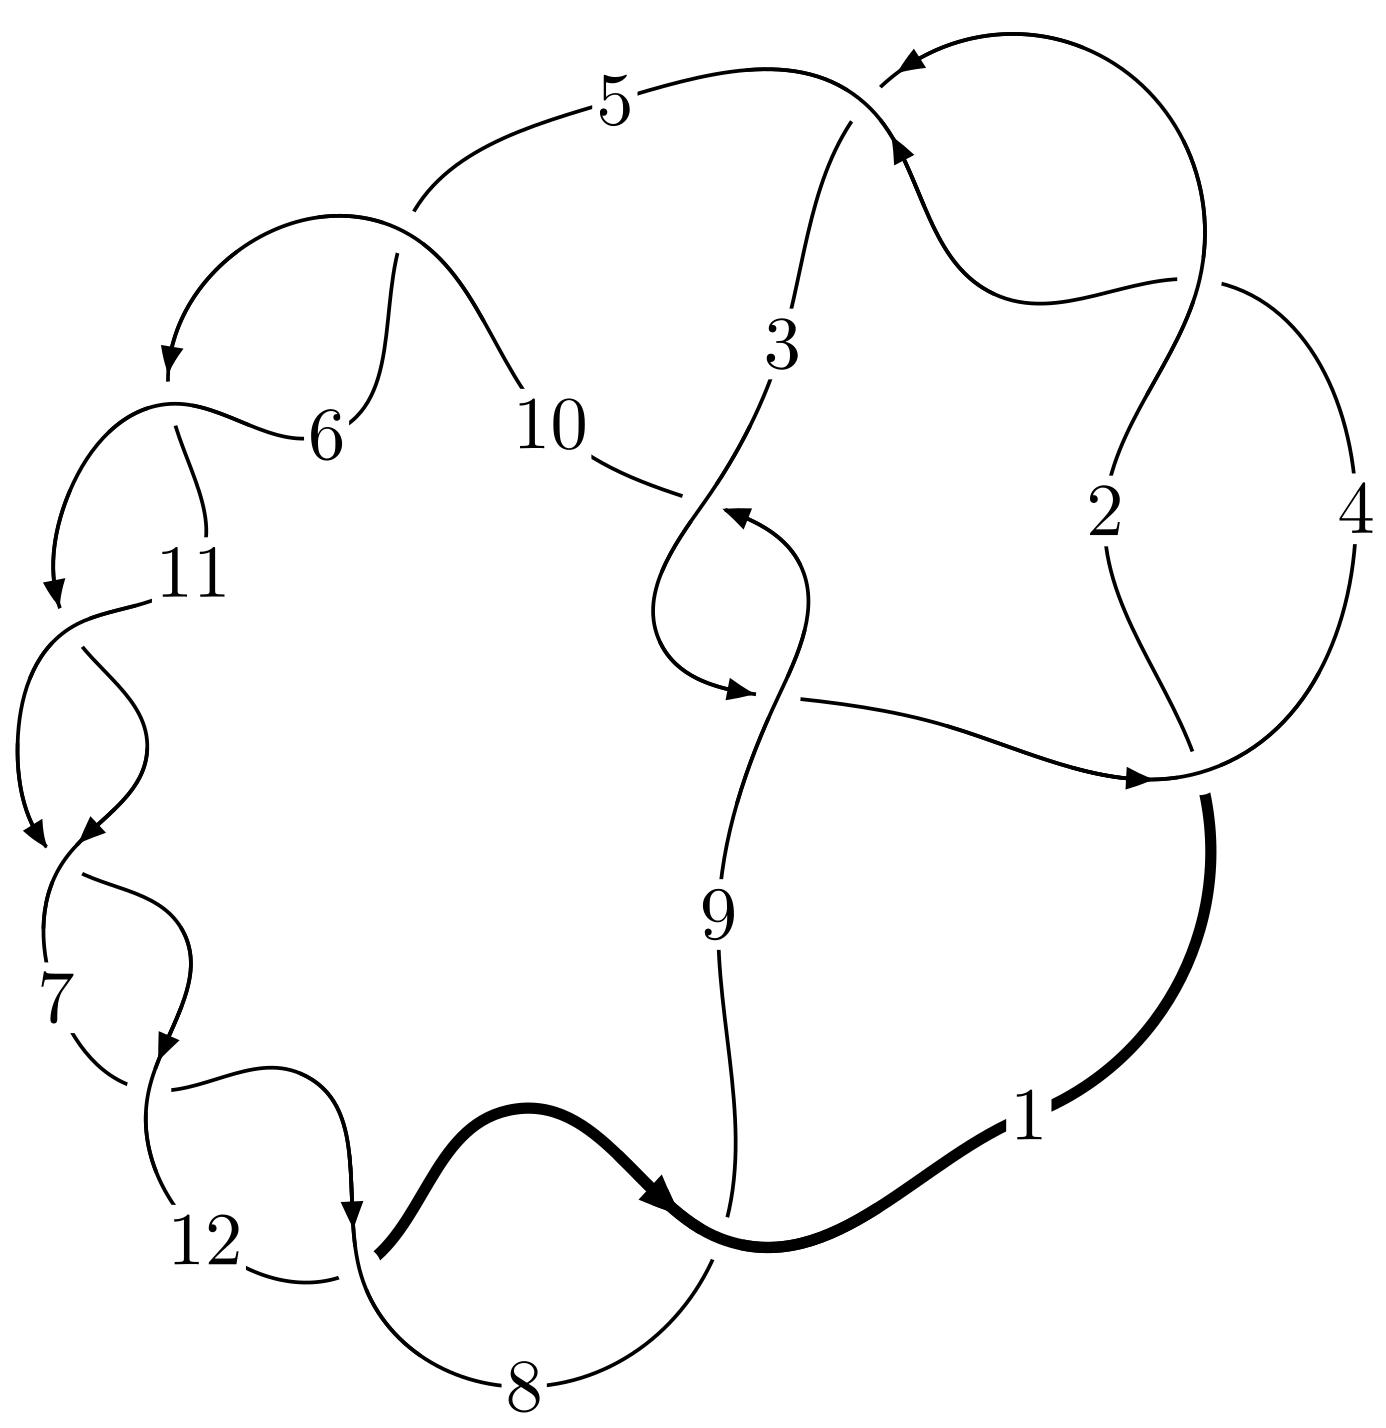
\includegraphics[width=112pt]{../../../GIT/diagram.site/Diagrams/png/1639_12a_0838.png}\\
\ \ \ A knot diagram\footnotemark}&
\allowdisplaybreaks
\textbf{Linearized knot diagam} \\
\cline{2-2}
 &
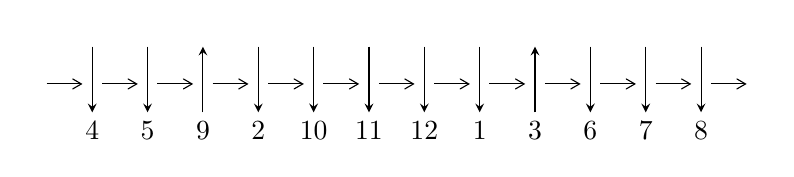
\begin{tikzpicture}[x=20pt, y=17pt]
	% nodes
	\node (C0) at (0, 0) {};
	\node (C1) at (1, 0) {};
	\node (C1U) at (1, +1) {};
	\node (C1D) at (1, -1) {4};

	\node (C2) at (2, 0) {};
	\node (C2U) at (2, +1) {};
	\node (C2D) at (2, -1) {5};

	\node (C3) at (3, 0) {};
	\node (C3U) at (3, +1) {};
	\node (C3D) at (3, -1) {9};

	\node (C4) at (4, 0) {};
	\node (C4U) at (4, +1) {};
	\node (C4D) at (4, -1) {2};

	\node (C5) at (5, 0) {};
	\node (C5U) at (5, +1) {};
	\node (C5D) at (5, -1) {10};

	\node (C6) at (6, 0) {};
	\node (C6U) at (6, +1) {};
	\node (C6D) at (6, -1) {11};

	\node (C7) at (7, 0) {};
	\node (C7U) at (7, +1) {};
	\node (C7D) at (7, -1) {12};

	\node (C8) at (8, 0) {};
	\node (C8U) at (8, +1) {};
	\node (C8D) at (8, -1) {1};

	\node (C9) at (9, 0) {};
	\node (C9U) at (9, +1) {};
	\node (C9D) at (9, -1) {3};

	\node (C10) at (10, 0) {};
	\node (C10U) at (10, +1) {};
	\node (C10D) at (10, -1) {6};

	\node (C11) at (11, 0) {};
	\node (C11U) at (11, +1) {};
	\node (C11D) at (11, -1) {7};

	\node (C12) at (12, 0) {};
	\node (C12U) at (12, +1) {};
	\node (C12D) at (12, -1) {8};
	\node (C13) at (13, 0) {};

	% arrows
	\draw[->,>={angle 60}]
	(C0) edge (C1) (C1) edge (C2) (C2) edge (C3) (C3) edge (C4) (C4) edge (C5) (C5) edge (C6) (C6) edge (C7) (C7) edge (C8) (C8) edge (C9) (C9) edge (C10) (C10) edge (C11) (C11) edge (C12) (C12) edge (C13) ;	\draw[->,>=stealth]
	(C1U) edge (C1D) (C2U) edge (C2D) (C3D) edge (C3U) (C4U) edge (C4D) (C5U) edge (C5D) (C6U) edge (C6D) (C7U) edge (C7D) (C8U) edge (C8D) (C9D) edge (C9U) (C10U) edge (C10D) (C11U) edge (C11D) (C12U) edge (C12D) ;
	\end{tikzpicture} \\
\hhline{~~} \\& 
\textbf{Solving Sequence} \\ \cline{2-2} 
 &
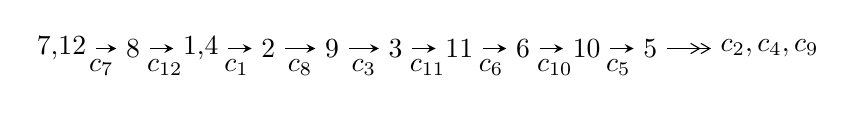
\begin{tikzpicture}[x=23pt, y=7pt]
	% node
	\node (A0) at (-1/8, 0) {7,12};
	\node (A1) at (1, 0) {8};
	\node (A2) at (33/16, 0) {1,4};
	\node (A3) at (25/8, 0) {2};
	\node (A4) at (33/8, 0) {9};
	\node (A5) at (41/8, 0) {3};
	\node (A6) at (49/8, 0) {11};
	\node (A7) at (57/8, 0) {6};
	\node (A8) at (65/8, 0) {10};
	\node (A9) at (73/8, 0) {5};
	\node (C1) at (1/2, -1) {$c_{7}$};
	\node (C2) at (3/2, -1) {$c_{12}$};
	\node (C3) at (21/8, -1) {$c_{1}$};
	\node (C4) at (29/8, -1) {$c_{8}$};
	\node (C5) at (37/8, -1) {$c_{3}$};
	\node (C6) at (45/8, -1) {$c_{11}$};
	\node (C7) at (53/8, -1) {$c_{6}$};
	\node (C8) at (61/8, -1) {$c_{10}$};
	\node (C9) at (69/8, -1) {$c_{5}$};
	\node (A10) at (11, 0) {$c_{2},c_{4},c_{9}$};

	% edge
	\draw[->,>=stealth]	
	(A0) edge (A1) (A1) edge (A2) (A2) edge (A3) (A3) edge (A4) (A4) edge (A5) (A5) edge (A6) (A6) edge (A7) (A7) edge (A8) (A8) edge (A9) ;
	\draw[->>,>={angle 60}]	
	(A9) edge (A10);
\end{tikzpicture} \\ 

\end{tabular} \\

\footnotetext{
The image of knot diagram is generated by the software ``\textbf{Draw programme}" developed by Andrew Bartholomew(\url{http://www.layer8.co.uk/maths/draw/index.htm\#Running-draw}), where we modified some parts for our purpose(\url{https://github.com/CATsTAILs/LinksPainter}).
}\phantom \\ \newline 
\centering \textbf{Ideals for irreducible components\footnotemark of $X_{\text{par}}$} 
 
\begin{align*}
I^u_{1}&=\langle 
u^{22}-17 u^{20}+\cdots+b+1,\;u^{22}+u^{21}+\cdots+a+2,\;u^{23}+2 u^{22}+\cdots-12 u^2+1\rangle \\
I^u_{2}&=\langle 
- u^2+b+1,\;- u^2+a+2,\;u^3- u^2-2 u+1\rangle \\
\\
\end{align*}
\raggedright * 2 irreducible components of $\dim_{\mathbb{C}}=0$, with total 26 representations.\\
\footnotetext{All coefficients of polynomials are rational numbers. But the coefficients are sometimes approximated in decimal forms when there is not enough margin.}
\newpage
\renewcommand{\arraystretch}{1}
\centering \section*{I. $I^u_{1}= \langle u^{22}-17 u^{20}+\cdots+b+1,\;u^{22}+u^{21}+\cdots+a+2,\;u^{23}+2 u^{22}+\cdots-12 u^2+1 \rangle$}
\flushleft \textbf{(i) Arc colorings}\\
\begin{tabular}{m{7pt} m{180pt} m{7pt} m{180pt} }
\flushright $a_{7}=$&$\begin{pmatrix}1\\0\end{pmatrix}$ \\
\flushright $a_{12}=$&$\begin{pmatrix}0\\u\end{pmatrix}$ \\
\flushright $a_{8}=$&$\begin{pmatrix}1\\u^2\end{pmatrix}$ \\
\flushright $a_{1}=$&$\begin{pmatrix}- u\\- u^3+u\end{pmatrix}$ \\
\flushright $a_{4}=$&$\begin{pmatrix}- u^{22}- u^{21}+\cdots+11 u-2\\- u^{22}+17 u^{20}+\cdots+2 u-1\end{pmatrix}$ \\
\flushright $a_{2}=$&$\begin{pmatrix}u^{21}-16 u^{19}+\cdots-11 u+2\\- u^{22}+16 u^{20}+\cdots+9 u^2- u\end{pmatrix}$ \\
\flushright $a_{9}=$&$\begin{pmatrix}- u^2+1\\- u^4+2 u^2\end{pmatrix}$ \\
\flushright $a_{3}=$&$\begin{pmatrix}u^{22}- u^{21}+\cdots+10 u-1\\3 u^{22}-48 u^{20}+\cdots+u+1\end{pmatrix}$ \\
\flushright $a_{11}=$&$\begin{pmatrix}u\\u\end{pmatrix}$ \\
\flushright $a_{6}=$&$\begin{pmatrix}- u^2+1\\- u^2\end{pmatrix}$ \\
\flushright $a_{10}=$&$\begin{pmatrix}- u^3+2 u\\- u^3+u\end{pmatrix}$ \\
\flushright $a_{5}=$&$\begin{pmatrix}u^4-3 u^2+1\\u^4-2 u^2\end{pmatrix}$\\&\end{tabular}
\flushleft \textbf{(ii) Obstruction class $= -1$}\\~\\
\flushleft \textbf{(iii) Cusp Shapes $= 5 u^{22}+8 u^{21}-81 u^{20}-126 u^{19}+556 u^{18}+835 u^{17}-2107 u^{16}-3020 u^{15}+4822 u^{14}+6443 u^{13}-6906 u^{12}-8110 u^{11}+6388 u^{10}+5547 u^9-4175 u^8-1464 u^7+2179 u^6-280 u^5-757 u^4+196 u^3+80 u^2-23 u-5$}\\~\\
\newpage\renewcommand{\arraystretch}{1}
\flushleft \textbf{(iv) u-Polynomials at the component}\newline \\
\begin{tabular}{m{50pt}|m{274pt}}
Crossings & \hspace{64pt}u-Polynomials at each crossing \\
\hline $$\begin{aligned}c_{1},c_{2},c_{4}\end{aligned}$$&$\begin{aligned}
&u^{23}-4 u^{22}+\cdots+5 u-1
\end{aligned}$\\
\hline $$\begin{aligned}c_{3},c_{9}\end{aligned}$$&$\begin{aligned}
&u^{23}- u^{22}+\cdots-28 u-8
\end{aligned}$\\
\hline $$\begin{aligned}c_{5},c_{6},c_{7}\\c_{8},c_{10},c_{11}\\c_{12}\end{aligned}$$&$\begin{aligned}
&u^{23}-2 u^{22}+\cdots+12 u^2-1
\end{aligned}$\\
\hline
\end{tabular}\\~\\
\newpage\renewcommand{\arraystretch}{1}
\flushleft \textbf{(v) Riley Polynomials at the component}\newline \\
\begin{tabular}{m{50pt}|m{274pt}}
Crossings & \hspace{64pt}Riley Polynomials at each crossing \\
\hline $$\begin{aligned}c_{1},c_{2},c_{4}\end{aligned}$$&$\begin{aligned}
&y^{23}-26 y^{22}+\cdots+57 y-1
\end{aligned}$\\
\hline $$\begin{aligned}c_{3},c_{9}\end{aligned}$$&$\begin{aligned}
&y^{23}+21 y^{22}+\cdots+592 y-64
\end{aligned}$\\
\hline $$\begin{aligned}c_{5},c_{6},c_{7}\\c_{8},c_{10},c_{11}\\c_{12}\end{aligned}$$&$\begin{aligned}
&y^{23}-36 y^{22}+\cdots+24 y-1
\end{aligned}$\\
\hline
\end{tabular}\\~\\
\newpage\flushleft \textbf{(vi) Complex Volumes and Cusp Shapes}
$$\begin{array}{c|c|c}  
\text{Solutions to }I^u_{1}& \I (\text{vol} + \sqrt{-1}CS) & \text{Cusp shape}\\
 \hline 
\begin{aligned}
u &= -0.899656 + 0.367597 I \\
a &= -0.129750 - 0.316248 I \\
b &= \phantom{-}1.37701 + 0.64432 I\end{aligned}
 & -10.62640 + 4.79693 I & -18.4963 - 4.5941 I \\ \hline\begin{aligned}
u &= -0.899656 - 0.367597 I \\
a &= -0.129750 + 0.316248 I \\
b &= \phantom{-}1.37701 - 0.64432 I\end{aligned}
 & -10.62640 - 4.79693 I & -18.4963 + 4.5941 I \\ \hline\begin{aligned}
u &= \phantom{-}0.869158\phantom{ +0.000000I} \\
a &= -0.611937\phantom{ +0.000000I} \\
b &= \phantom{-}1.66429\phantom{ +0.000000I}\end{aligned}
 & -5.48753\phantom{ +0.000000I} & -17.2890\phantom{ +0.000000I} \\ \hline\begin{aligned}
u &= -0.821958 + 0.135064 I \\
a &= -0.253247 + 1.039930 I \\
b &= -0.445233 + 0.309895 I\end{aligned}
 & -3.58507 + 2.11349 I & -17.2477 - 5.0037 I \\ \hline\begin{aligned}
u &= -0.821958 - 0.135064 I \\
a &= -0.253247 - 1.039930 I \\
b &= -0.445233 - 0.309895 I\end{aligned}
 & -3.58507 - 2.11349 I & -17.2477 + 5.0037 I \\ \hline\begin{aligned}
u &= -1.29295\phantom{ +0.000000I} \\
a &= -0.815349\phantom{ +0.000000I} \\
b &= -0.215176\phantom{ +0.000000I}\end{aligned}
 & -6.99093\phantom{ +0.000000I} & -10.8460\phantom{ +0.000000I} \\ \hline\begin{aligned}
u &= \phantom{-}0.292199 + 0.547469 I \\
a &= -0.70419 + 1.55774 I \\
b &= -0.871306 + 0.010708 I\end{aligned}
 & -6.92984 - 1.76193 I & -14.7690 + 3.3456 I \\ \hline\begin{aligned}
u &= \phantom{-}0.292199 - 0.547469 I \\
a &= -0.70419 - 1.55774 I \\
b &= -0.871306 - 0.010708 I\end{aligned}
 & -6.92984 + 1.76193 I & -14.7690 - 3.3456 I \\ \hline\begin{aligned}
u &= \phantom{-}1.43893 + 0.05540 I \\
a &= -0.573918 + 0.627821 I \\
b &= -0.269240 + 1.142030 I\end{aligned}
 & -11.26780 - 2.80601 I & -17.5990 + 3.0357 I \\ \hline\begin{aligned}
u &= \phantom{-}1.43893 - 0.05540 I \\
a &= -0.573918 - 0.627821 I \\
b &= -0.269240 - 1.142030 I\end{aligned}
 & -11.26780 + 2.80601 I & -17.5990 - 3.0357 I\\
 \hline 
 \end{array}$$\newpage$$\begin{array}{c|c|c}  
\text{Solutions to }I^u_{1}& \I (\text{vol} + \sqrt{-1}CS) & \text{Cusp shape}\\
 \hline 
\begin{aligned}
u &= -1.45875\phantom{ +0.000000I} \\
a &= \phantom{-}2.49389\phantom{ +0.000000I} \\
b &= \phantom{-}1.79311\phantom{ +0.000000I}\end{aligned}
 & -13.4340\phantom{ +0.000000I} & -18.2600\phantom{ +0.000000I} \\ \hline\begin{aligned}
u &= \phantom{-}0.523970\phantom{ +0.000000I} \\
a &= \phantom{-}0.174078\phantom{ +0.000000I} \\
b &= -0.424666\phantom{ +0.000000I}\end{aligned}
 & -0.880680\phantom{ +0.000000I} & -10.8440\phantom{ +0.000000I} \\ \hline\begin{aligned}
u &= \phantom{-}1.46882 + 0.17141 I \\
a &= \phantom{-}1.75548 - 0.96316 I \\
b &= \phantom{-}1.371010 - 0.251551 I\end{aligned}
 & -18.5944 - 6.8465 I & -19.2959 + 3.6692 I \\ \hline\begin{aligned}
u &= \phantom{-}1.46882 - 0.17141 I \\
a &= \phantom{-}1.75548 + 0.96316 I \\
b &= \phantom{-}1.371010 + 0.251551 I\end{aligned}
 & -18.5944 + 6.8465 I & -19.2959 - 3.6692 I \\ \hline\begin{aligned}
u &= \phantom{-}0.198961 + 0.259775 I \\
a &= \phantom{-}1.162630 + 0.050871 I \\
b &= \phantom{-}0.098000 - 0.372398 I\end{aligned}
 & -0.444837 - 0.821194 I & -9.62649 + 8.14856 I \\ \hline\begin{aligned}
u &= \phantom{-}0.198961 - 0.259775 I \\
a &= \phantom{-}1.162630 - 0.050871 I \\
b &= \phantom{-}0.098000 + 0.372398 I\end{aligned}
 & -0.444837 + 0.821194 I & -9.62649 - 8.14856 I \\ \hline\begin{aligned}
u &= -0.236506\phantom{ +0.000000I} \\
a &= -3.87954\phantom{ +0.000000I} \\
b &= -0.871608\phantom{ +0.000000I}\end{aligned}
 & -1.99765\phantom{ +0.000000I} & \phantom{-}0.552820\phantom{ +0.000000I} \\ \hline\begin{aligned}
u &= \phantom{-}1.81292\phantom{ +0.000000I} \\
a &= \phantom{-}1.34454\phantom{ +0.000000I} \\
b &= \phantom{-}2.75785\phantom{ +0.000000I}\end{aligned}
 & -18.5335\phantom{ +0.000000I} & -9.99140\phantom{ +0.000000I} \\ \hline\begin{aligned}
u &= -1.85429 + 0.01361 I \\
a &= \phantom{-}1.048680 + 0.206116 I \\
b &= \phantom{-}2.22063 + 0.96437 I\end{aligned}
 & \phantom{-}15.7173 + 3.1639 I & -17.6160 - 2.4156 I \\ \hline\begin{aligned}
u &= -1.85429 - 0.01361 I \\
a &= \phantom{-}1.048680 - 0.206116 I \\
b &= \phantom{-}2.22063 - 0.96437 I\end{aligned}
 & \phantom{-}15.7173 - 3.1639 I & -17.6160 + 2.4156 I\\
 \hline 
 \end{array}$$\newpage$$\begin{array}{c|c|c}  
\text{Solutions to }I^u_{1}& \I (\text{vol} + \sqrt{-1}CS) & \text{Cusp shape}\\
 \hline 
\begin{aligned}
u &= \phantom{-}1.85896\phantom{ +0.000000I} \\
a &= -3.64519\phantom{ +0.000000I} \\
b &= -8.09850\phantom{ +0.000000I}\end{aligned}
 & \phantom{-}13.4167\phantom{ +0.000000I} & -18.4390\phantom{ +0.000000I} \\ \hline\begin{aligned}
u &= -1.86140 + 0.04356 I \\
a &= -2.83593 - 1.10657 I \\
b &= -6.28352 - 2.42136 I\end{aligned}
 & \phantom{-}8.27161 + 7.98934 I & -19.2912 - 3.1659 I \\ \hline\begin{aligned}
u &= -1.86140 - 0.04356 I \\
a &= -2.83593 + 1.10657 I \\
b &= -6.28352 + 2.42136 I\end{aligned}
 & \phantom{-}8.27161 - 7.98934 I & -19.2912 + 3.1659 I\\
 \hline 
 \end{array}$$\newpage\newpage\renewcommand{\arraystretch}{1}
\centering \section*{II. $I^u_{2}= \langle - u^2+b+1,\;- u^2+a+2,\;u^3- u^2-2 u+1 \rangle$}
\flushleft \textbf{(i) Arc colorings}\\
\begin{tabular}{m{7pt} m{180pt} m{7pt} m{180pt} }
\flushright $a_{7}=$&$\begin{pmatrix}1\\0\end{pmatrix}$ \\
\flushright $a_{12}=$&$\begin{pmatrix}0\\u\end{pmatrix}$ \\
\flushright $a_{8}=$&$\begin{pmatrix}1\\u^2\end{pmatrix}$ \\
\flushright $a_{1}=$&$\begin{pmatrix}- u\\- u^2- u+1\end{pmatrix}$ \\
\flushright $a_{4}=$&$\begin{pmatrix}u^2-2\\u^2-1\end{pmatrix}$ \\
\flushright $a_{2}=$&$\begin{pmatrix}u^2- u-2\\- u\end{pmatrix}$ \\
\flushright $a_{9}=$&$\begin{pmatrix}- u^2+1\\- u^2- u+1\end{pmatrix}$ \\
\flushright $a_{3}=$&$\begin{pmatrix}u^2-2\\u^2-1\end{pmatrix}$ \\
\flushright $a_{11}=$&$\begin{pmatrix}u\\u\end{pmatrix}$ \\
\flushright $a_{6}=$&$\begin{pmatrix}- u^2+1\\- u^2\end{pmatrix}$ \\
\flushright $a_{10}=$&$\begin{pmatrix}- u^2+1\\- u^2- u+1\end{pmatrix}$ \\
\flushright $a_{5}=$&$\begin{pmatrix}u\\u^2+u-1\end{pmatrix}$\\&\end{tabular}
\flushleft \textbf{(ii) Obstruction class $= 1$}\\~\\
\flushleft \textbf{(iii) Cusp Shapes $= u^2- u-23$}\\~\\
\newpage\renewcommand{\arraystretch}{1}
\flushleft \textbf{(iv) u-Polynomials at the component}\newline \\
\begin{tabular}{m{50pt}|m{274pt}}
Crossings & \hspace{64pt}u-Polynomials at each crossing \\
\hline $$\begin{aligned}c_{1},c_{2}\end{aligned}$$&$\begin{aligned}
&(u-1)^3
\end{aligned}$\\
\hline $$\begin{aligned}c_{3},c_{9}\end{aligned}$$&$\begin{aligned}
&u^3
\end{aligned}$\\
\hline $$\begin{aligned}c_{4}\end{aligned}$$&$\begin{aligned}
&(u+1)^3
\end{aligned}$\\
\hline $$\begin{aligned}c_{5},c_{6},c_{7}\\c_{8}\end{aligned}$$&$\begin{aligned}
&u^3- u^2-2 u+1
\end{aligned}$\\
\hline $$\begin{aligned}c_{10},c_{11},c_{12}\end{aligned}$$&$\begin{aligned}
&u^3+u^2-2 u-1
\end{aligned}$\\
\hline
\end{tabular}\\~\\
\newpage\renewcommand{\arraystretch}{1}
\flushleft \textbf{(v) Riley Polynomials at the component}\newline \\
\begin{tabular}{m{50pt}|m{274pt}}
Crossings & \hspace{64pt}Riley Polynomials at each crossing \\
\hline $$\begin{aligned}c_{1},c_{2},c_{4}\end{aligned}$$&$\begin{aligned}
&(y-1)^3
\end{aligned}$\\
\hline $$\begin{aligned}c_{3},c_{9}\end{aligned}$$&$\begin{aligned}
&y^3
\end{aligned}$\\
\hline $$\begin{aligned}c_{5},c_{6},c_{7}\\c_{8},c_{10},c_{11}\\c_{12}\end{aligned}$$&$\begin{aligned}
&y^3-5 y^2+6 y-1
\end{aligned}$\\
\hline
\end{tabular}\\~\\
\newpage\flushleft \textbf{(vi) Complex Volumes and Cusp Shapes}
$$\begin{array}{c|c|c}  
\text{Solutions to }I^u_{2}& \I (\text{vol} + \sqrt{-1}CS) & \text{Cusp shape}\\
 \hline 
\begin{aligned}
u &= -1.24698\phantom{ +0.000000I} \\
a &= -0.445042\phantom{ +0.000000I} \\
b &= \phantom{-}0.554958\phantom{ +0.000000I}\end{aligned}
 & -7.98968\phantom{ +0.000000I} & -20.1980\phantom{ +0.000000I} \\ \hline\begin{aligned}
u &= \phantom{-}0.445042\phantom{ +0.000000I} \\
a &= -1.80194\phantom{ +0.000000I} \\
b &= -0.801938\phantom{ +0.000000I}\end{aligned}
 & -2.34991\phantom{ +0.000000I} & -23.2470\phantom{ +0.000000I} \\ \hline\begin{aligned}
u &= \phantom{-}1.80194\phantom{ +0.000000I} \\
a &= \phantom{-}1.24698\phantom{ +0.000000I} \\
b &= \phantom{-}2.24698\phantom{ +0.000000I}\end{aligned}
 & -19.2692\phantom{ +0.000000I} & -21.5550\phantom{ +0.000000I}\\
 \hline 
 \end{array}$$\newpage
\newpage\renewcommand{\arraystretch}{1}
\centering \section*{ III. u-Polynomials}
\begin{tabular}{m{50pt}|m{274pt}}
Crossings & \hspace{64pt}u-Polynomials at each crossing \\
\hline $$\begin{aligned}c_{1},c_{2}\end{aligned}$$&$\begin{aligned}
&((u-1)^3)(u^{23}-4 u^{22}+\cdots+5 u-1)
\end{aligned}$\\
\hline $$\begin{aligned}c_{3},c_{9}\end{aligned}$$&$\begin{aligned}
&u^3(u^{23}- u^{22}+\cdots-28 u-8)
\end{aligned}$\\
\hline $$\begin{aligned}c_{4}\end{aligned}$$&$\begin{aligned}
&((u+1)^3)(u^{23}-4 u^{22}+\cdots+5 u-1)
\end{aligned}$\\
\hline $$\begin{aligned}c_{5},c_{6},c_{7}\\c_{8}\end{aligned}$$&$\begin{aligned}
&(u^3- u^2-2 u+1)(u^{23}-2 u^{22}+\cdots+12 u^2-1)
\end{aligned}$\\
\hline $$\begin{aligned}c_{10},c_{11},c_{12}\end{aligned}$$&$\begin{aligned}
&(u^3+u^2-2 u-1)(u^{23}-2 u^{22}+\cdots+12 u^2-1)
\end{aligned}$\\
\hline
\end{tabular}\newpage\renewcommand{\arraystretch}{1}
\centering \section*{ IV. Riley Polynomials}
\begin{tabular}{m{50pt}|m{274pt}}
Crossings & \hspace{64pt}Riley Polynomials at each crossing \\
\hline $$\begin{aligned}c_{1},c_{2},c_{4}\end{aligned}$$&$\begin{aligned}
&((y-1)^3)(y^{23}-26 y^{22}+\cdots+57 y-1)
\end{aligned}$\\
\hline $$\begin{aligned}c_{3},c_{9}\end{aligned}$$&$\begin{aligned}
&y^3(y^{23}+21 y^{22}+\cdots+592 y-64)
\end{aligned}$\\
\hline $$\begin{aligned}c_{5},c_{6},c_{7}\\c_{8},c_{10},c_{11}\\c_{12}\end{aligned}$$&$\begin{aligned}
&(y^3-5 y^2+6 y-1)(y^{23}-36 y^{22}+\cdots+24 y-1)
\end{aligned}$\\
\hline
\end{tabular}
\vskip 2pc
\end{document}